\chapter{Results}
\section{Yields and kinematic distributions}
After the selections described in Section \ref{sec:event_selection}, the event yields are extracted for signal and backgrounds for each of the four periods of Run2, for the signal and control regions.
The pre-fit yields for the signal and background processes for the signal region SR4P\_1P, can be seen in Table \ref{tab:Run2_SR4P_phoCR_lepCR}.
Additional tables, including also the observed number of data events, are provided for the fake photons application region (Table \ref{tab:yields_Run2_CR4P_1F_lepCR}), and for the fake leptons application regions (Tables \ref{tab:yields_Run2_CR3P1F_1P}, \ref{tab:yields_Run2_CR2P2F_1P})

\begin{table}
\caption{Yields from the signal region SR4P\_1P, with four leptons passing the tight selection and a photon passing the cut-based ID.}
\label{tab:Run2_SR4P_phoCR_lepCR}
% Note: this is from the variable mZZGloose
\resizebox{\textwidth}{!}{%
\begin{tabular}{lrrrrr}
\toprule
{} & \multicolumn{1}{c}{2016preVFP} & \multicolumn{1}{c}{2016postVFP} & \multicolumn{1}{c}{2017} & \multicolumn{1}{c}{2018} & \multicolumn{1}{c}{Run2} \\
\midrule
ZZGTo4LG-prompt  &  1.889 $\pm$ 0.046 &  1.657 $\pm$ 0.040 &  3.812 $\pm$ 0.097 &   5.480 $\pm$ 0.137 &  12.838 $\pm$ 0.178 \\
ZZTo4l-prompt    &  1.185 $\pm$ 0.023 &  1.093 $\pm$ 0.021 &  2.559 $\pm$ 0.036 &   3.710 $\pm$ 0.052 &   8.546 $\pm$ 0.071 \\
ggTo4e-prompt    &  0.030 $\pm$ 0.001 &  0.029 $\pm$ 0.001 &  0.072 $\pm$ 0.002 &   0.101 $\pm$ 0.003 &   0.232 $\pm$ 0.004 \\
ggTo2e2mu-prompt &  0.062 $\pm$ 0.003 &  0.056 $\pm$ 0.002 &  0.066 $\pm$ 0.003 &   0.102 $\pm$ 0.004 &   0.286 $\pm$ 0.006 \\
ggTo4mu-prompt   &  0.056 $\pm$ 0.001 &  0.046 $\pm$ 0.001 &  0.113 $\pm$ 0.003 &   0.153 $\pm$ 0.004 &   0.368 $\pm$ 0.005 \\
ZZZ-prompt       &  0.007 $\pm$ 0.005 &  0.000 $\pm$ 0.000 &  0.017 $\pm$ 0.008 &   0.029 $\pm$ 0.010 &   0.053 $\pm$ 0.014 \\
TTZJets-prompt   &  0.010 $\pm$ 0.002 &  0.009 $\pm$ 0.002 &  0.034 $\pm$ 0.005 &   0.040 $\pm$ 0.006 &   0.094 $\pm$ 0.008 \\
fake\_photons     &  1.212 $\pm$ 0.638 &  0.710 $\pm$ 0.411 &  1.195 $\pm$ 0.489 &   1.736 $\pm$ 0.588 &   4.853 $\pm$ 1.077 \\
WZZ-prompt       &  0.000 $\pm$ 0.000 &  0.014 $\pm$ 0.010 &  0.017 $\pm$ 0.016 &   0.053 $\pm$ 0.024 &   0.085 $\pm$ 0.031 \\
WWZ-prompt       &  0.000 $\pm$ 0.000 &  0.040 $\pm$ 0.040 &  0.041 $\pm$ 0.041 &   0.082 $\pm$ 0.058 &   0.163 $\pm$ 0.081 \\
\midrule
Total            &  4.451 $\pm$ 0.640 &  3.653 $\pm$ 0.415 &  7.927 $\pm$ 0.502 &  11.485 $\pm$ 0.609 &  27.517 $\pm$ 1.098 \\
\bottomrule
\end{tabular}
}
\end{table}

\begin{table}
\caption{Yields from the fake photon application region CR4P\_1F, with four leptons passing the tight selection and a photon passing the VeryLoose ID but failing the cut-based ID Loose.}
\label{tab:yields_Run2_CR4P_1F_lepCR}
\resizebox{\textwidth}{!}{%
\begin{tabular}{lrrrrr}
\toprule
{} & \multicolumn{1}{c}{2016preVFP} & \multicolumn{1}{c}{2016postVFP} & \multicolumn{1}{c}{2017} & \multicolumn{1}{c}{2018} & \multicolumn{1}{c}{Run2} \\
\midrule
ZZGTo4LG  &  0.286 $\pm$ 0.019 &  0.270 $\pm$ 0.016 &  0.751 $\pm$ 0.044 &   1.061 $\pm$ 0.060 &   2.367 $\pm$ 0.078 \\
ZZTo4l    &  2.270 $\pm$ 0.032 &  2.162 $\pm$ 0.029 &  6.228 $\pm$ 0.057 &   9.118 $\pm$ 0.082 &  19.777 $\pm$ 0.108 \\
ggTo4e    &  0.050 $\pm$ 0.001 &  0.048 $\pm$ 0.001 &  0.137 $\pm$ 0.003 &   0.203 $\pm$ 0.004 &   0.438 $\pm$ 0.005 \\
ggTo2e2mu &  0.131 $\pm$ 0.004 &  0.128 $\pm$ 0.004 &  0.180 $\pm$ 0.005 &   0.253 $\pm$ 0.007 &   0.691 $\pm$ 0.010 \\
ggTo4mu   &  0.088 $\pm$ 0.002 &  0.075 $\pm$ 0.001 &  0.202 $\pm$ 0.004 &   0.305 $\pm$ 0.006 &   0.671 $\pm$ 0.007 \\
ZZZ       &  0.039 $\pm$ 0.011 &  0.018 $\pm$ 0.009 &  0.057 $\pm$ 0.015 &   0.066 $\pm$ 0.018 &   0.180 $\pm$ 0.027 \\
WZZ       &  0.051 $\pm$ 0.020 &  0.051 $\pm$ 0.019 &  0.077 $\pm$ 0.028 &   0.120 $\pm$ 0.038 &   0.299 $\pm$ 0.055 \\
WWZ       &  0.048 $\pm$ 0.048 &  0.046 $\pm$ 0.046 &  0.000 $\pm$ 0.000 &   0.000 $\pm$ 0.000 &   0.094 $\pm$ 0.067 \\
TTZJets   &  0.046 $\pm$ 0.005 &  0.039 $\pm$ 0.004 &  0.144 $\pm$ 0.010 &   0.216 $\pm$ 0.014 &   0.444 $\pm$ 0.019 \\
\midrule
Total     &  3.008 $\pm$ 0.066 &  2.836 $\pm$ 0.061 &  7.776 $\pm$ 0.079 &  11.342 $\pm$ 0.111 &  24.962 $\pm$ 0.163 \\
Data      & \multicolumn{1}{c}{4} & \multicolumn{1}{c}{3} & \multicolumn{1}{c}{6} & \multicolumn{1}{c}{9} & \multicolumn{1}{c}{22} \\
\bottomrule
\end{tabular}
}
\end{table}

\begin{table}
\caption{Yields in CR3P1F\_1P, one of the fake lepton application regions, with three leptons passing the tight selection, one passing only a loose selection, and a photon passing the cut-based ID.}
\label{tab:yields_Run2_CR3P1F_1P}
\resizebox{\textwidth}{!}{%
\begin{tabular}{lrrrrr}
\toprule
{} & \multicolumn{1}{c}{2016preVFP} & \multicolumn{1}{c}{2016postVFP} & \multicolumn{1}{c}{2017} & \multicolumn{1}{c}{2018} & \multicolumn{1}{c}{Run2} \\
\midrule
ZZGTo4LG       &  0.126 $\pm$ 0.013 &  0.131 $\pm$ 0.011 &  0.369 $\pm$ 0.031 &  0.453 $\pm$ 0.039 &  1.080 $\pm$ 0.052 \\
WZGTo3LNuG     &  0.203 $\pm$ 0.010 &  0.185 $\pm$ 0.008 &  0.392 $\pm$ 0.019 &  0.673 $\pm$ 0.030 &  1.453 $\pm$ 0.038 \\
ZGToLLG        &  0.695 $\pm$ 0.280 &  0.000 $\pm$ 0.000 &  0.463 $\pm$ 0.388 &  0.492 $\pm$ 0.447 &  1.650 $\pm$ 0.654 \\
ZZTo4l         &  0.179 $\pm$ 0.009 &  0.160 $\pm$ 0.008 &  0.412 $\pm$ 0.015 &  0.618 $\pm$ 0.021 &  1.368 $\pm$ 0.029 \\
ggTo4e         &  0.008 $\pm$ 0.000 &  0.006 $\pm$ 0.000 &  0.017 $\pm$ 0.001 &  0.029 $\pm$ 0.002 &  0.061 $\pm$ 0.002 \\
ggTo2e2mu      &  0.011 $\pm$ 0.001 &  0.009 $\pm$ 0.001 &  0.012 $\pm$ 0.001 &  0.018 $\pm$ 0.002 &  0.049 $\pm$ 0.003 \\
ggTo4mu        &  0.003 $\pm$ 0.000 &  0.002 $\pm$ 0.000 &  0.006 $\pm$ 0.001 &  0.007 $\pm$ 0.001 &  0.019 $\pm$ 0.001 \\
WZTo3LNu       &  0.359 $\pm$ 0.103 &  0.434 $\pm$ 0.093 &  0.500 $\pm$ 0.174 &  1.055 $\pm$ 0.316 &  2.348 $\pm$ 0.387 \\
ZZZ            &  0.003 $\pm$ 0.003 &  0.000 $\pm$ 0.000 &  0.010 $\pm$ 0.006 &  0.007 $\pm$ 0.005 &  0.020 $\pm$ 0.008 \\
WZZ            &  0.009 $\pm$ 0.009 &  0.000 $\pm$ 0.000 &  0.001 $\pm$ 0.012 &  0.012 $\pm$ 0.012 &  0.022 $\pm$ 0.019 \\
TTZJets        &  0.035 $\pm$ 0.004 &  0.032 $\pm$ 0.004 &  0.060 $\pm$ 0.006 &  0.107 $\pm$ 0.010 &  0.235 $\pm$ 0.013 \\
DYJetsToLL\_M50&  0.000 $\pm$ 0.000 &  0.000 $\pm$ 0.000 &  0.000 $\pm$ 0.000 &  0.680 $\pm$ 3.520 &  0.680 $\pm$ 3.520 \\
\midrule
Total          &  1.631 $\pm$ 0.299 &  0.960 $\pm$ 0.095 &  2.242 $\pm$ 0.427 &  4.152 $\pm$ 3.562 &  8.985 $\pm$ 3.602 \\
Data & \multicolumn{1}{c}{1} & \multicolumn{1}{c}{0} & \multicolumn{1}{c}{2} & \multicolumn{1}{c}{4} & \multicolumn{1}{c}{7} \\
\bottomrule
\end{tabular}
}
\end{table}

\begin{table}
\caption{Yields in CR2P2F\_1P, one of the fake lepton application regions, with two leptons passing the tight selection, two passing only a loose selection, and a photon passing the cut-based ID.}
\label{tab:yields_Run2_CR2P2F_1P}
\resizebox{\textwidth}{!}{%
\begin{tabular}{lrrrrr}
\toprule
{} & \multicolumn{1}{c}{2016preVFP} & \multicolumn{1}{c}{2016postVFP} & \multicolumn{1}{c}{2017} & \multicolumn{1}{c}{2018} & \multicolumn{1}{c}{Run2} \\
\midrule
ZZGTo4LG       &   0.008 $\pm$ 0.004 &   0.005 $\pm$ 0.002 &    0.006 $\pm$ 0.004 &    0.030 $\pm$ 0.010 &    0.050 $\pm$ 0.011 \\
WZGTo3LNuG     &   0.022 $\pm$ 0.003 &   0.019 $\pm$ 0.003 &    0.032 $\pm$ 0.005 &    0.048 $\pm$ 0.008 &    0.121 $\pm$ 0.011 \\
ZGToLLG        &   6.473 $\pm$ 0.786 &   0.000 $\pm$ 0.000 &   13.535 $\pm$ 1.451 &   20.784 $\pm$ 2.258 &   40.792 $\pm$ 2.796 \\
ZZTo4l         &   0.013 $\pm$ 0.003 &   0.011 $\pm$ 0.002 &    0.017 $\pm$ 0.003 &    0.032 $\pm$ 0.005 &    0.074 $\pm$ 0.007 \\
ggTo4e         &   0.000 $\pm$ 0.000 &   0.000 $\pm$ 0.000 &    0.000 $\pm$ 0.000 &    0.001 $\pm$ 0.000 &    0.001 $\pm$ 0.000 \\
ggTo2e2mu      &   0.000 $\pm$ 0.000 &   0.000 $\pm$ 0.000 &    0.000 $\pm$ 0.000 &    0.000 $\pm$ 0.000 &    0.001 $\pm$ 0.000 \\
WZTo3LNu       &   0.018 $\pm$ 0.035 &   0.052 $\pm$ 0.041 &    0.185 $\pm$ 0.108 &    0.238 $\pm$ 0.121 &    0.493 $\pm$ 0.171 \\
TTZJets        &   0.020 $\pm$ 0.003 &   0.017 $\pm$ 0.003 &    0.029 $\pm$ 0.004 &    0.043 $\pm$ 0.006 &    0.110 $\pm$ 0.009 \\
TZq            &   0.005 $\pm$ 0.007 &   0.000 $\pm$ 0.006 &    0.018 $\pm$ 0.009 &    0.021 $\pm$ 0.012 &    0.044 $\pm$ 0.018 \\
tW             &   0.057 $\pm$ 0.057 &   0.000 $\pm$ 0.000 &    0.088 $\pm$ 0.099 &    0.000 $\pm$ 0.000 &    0.144 $\pm$ 0.114 \\
DYJetsToLL\_M50 &   0.000 $\pm$ 0.000 &  11.019 $\pm$ 6.842 &  14.447 $\pm$ 10.750 &  29.521 $\pm$ 14.716 &  54.986 $\pm$ 19.467 \\
ggTo4mu        &   0.000 $\pm$ 0.000 &   0.000 $\pm$ 0.000 &    0.000 $\pm$ 0.000 &    0.000 $\pm$ 0.000 &    0.000 $\pm$ 0.000 \\
\midrule
Total          &   6.616 $\pm$ 0.789 &  11.123 $\pm$ 6.842 &  28.359 $\pm$ 10.849 &  50.717 $\pm$ 14.889 &  96.814 $\pm$ 19.667 \\
Data & \multicolumn{1}{c}{17} & \multicolumn{1}{c}{8} & \multicolumn{1}{c}{21} & \multicolumn{1}{c}{22} & \multicolumn{1}{c}{68} \\
\bottomrule
\end{tabular}
}
\end{table}

\begin{figure}
\subfigure [2016preVFP ] {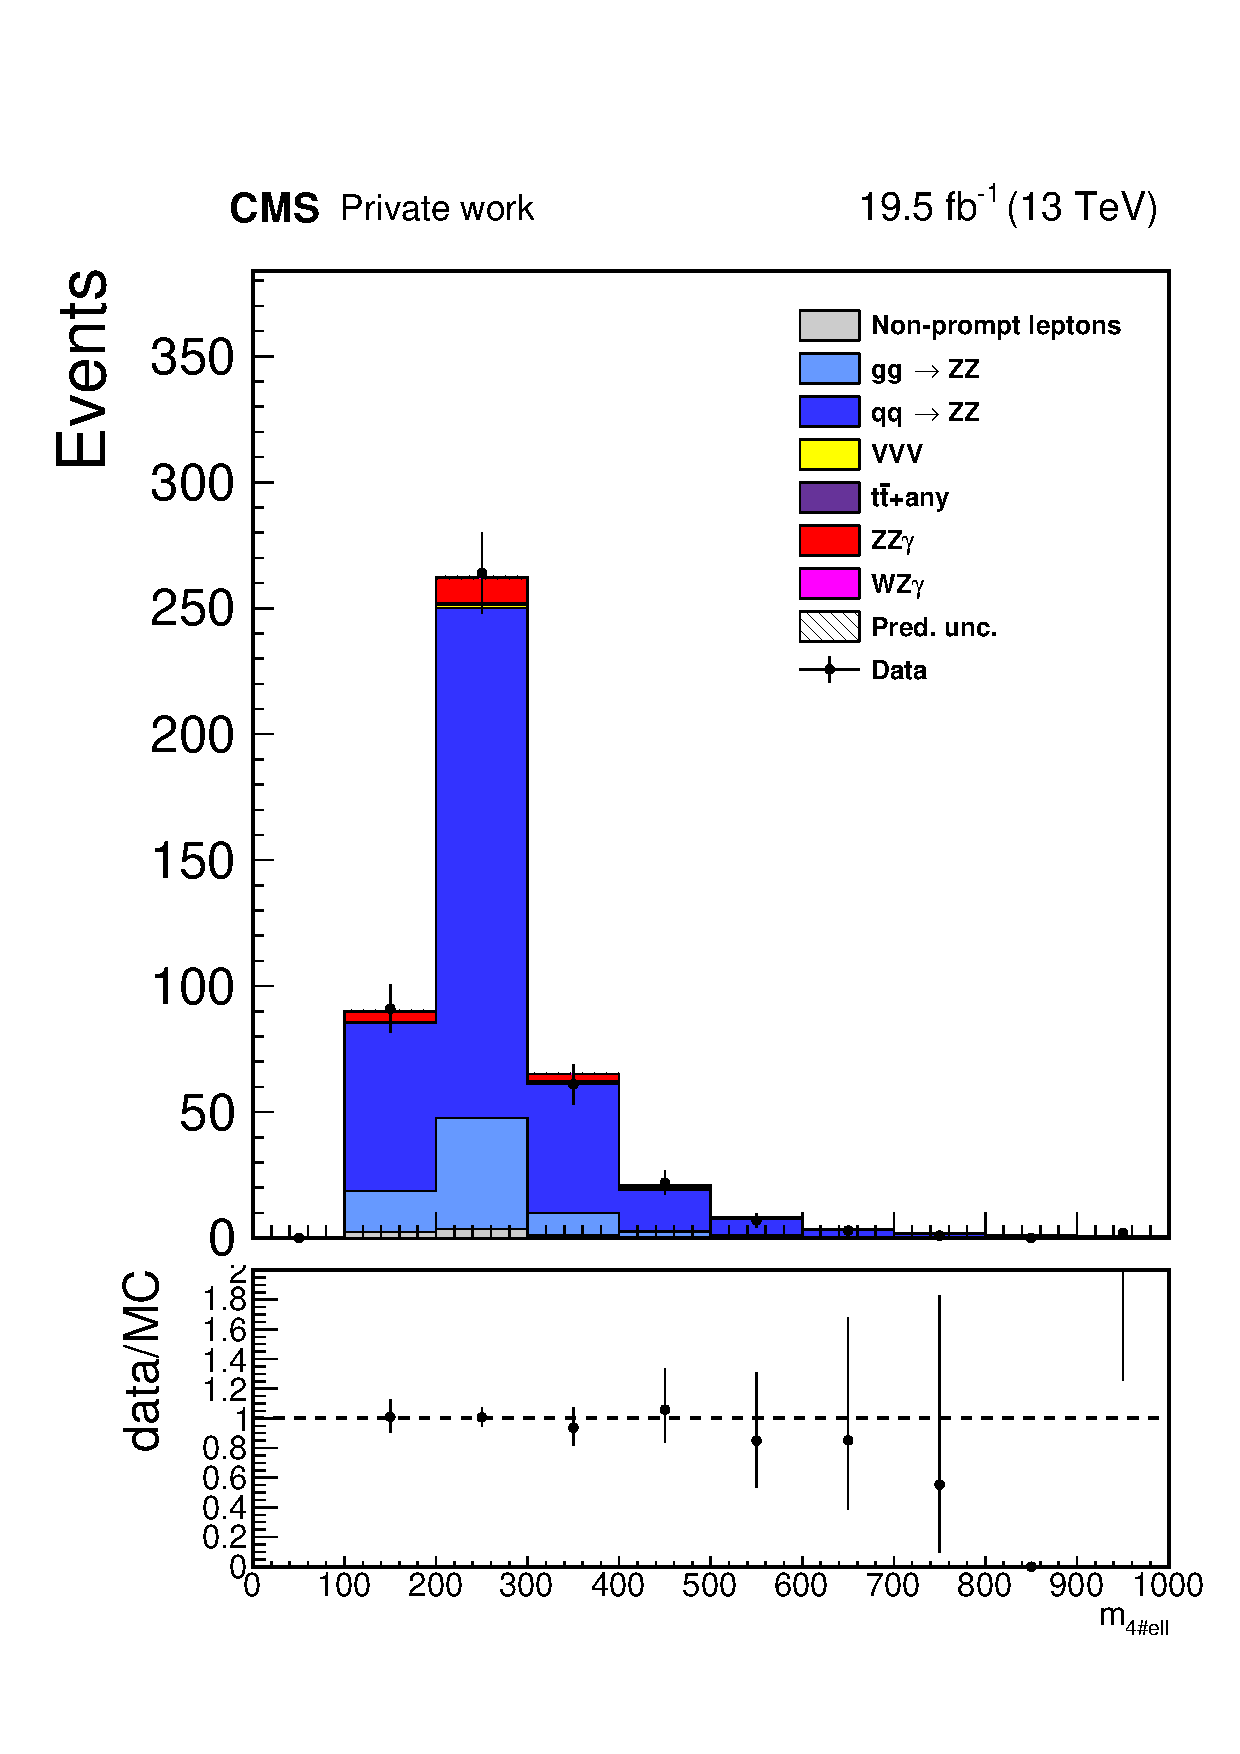
\includegraphics[width=.25\textwidth]{Figures/VVGammaAnalyzer/2016preVFP/lepCR/SR4P/ZZ_mass_pow.pdf}}%
\subfigure [2016postVFP] {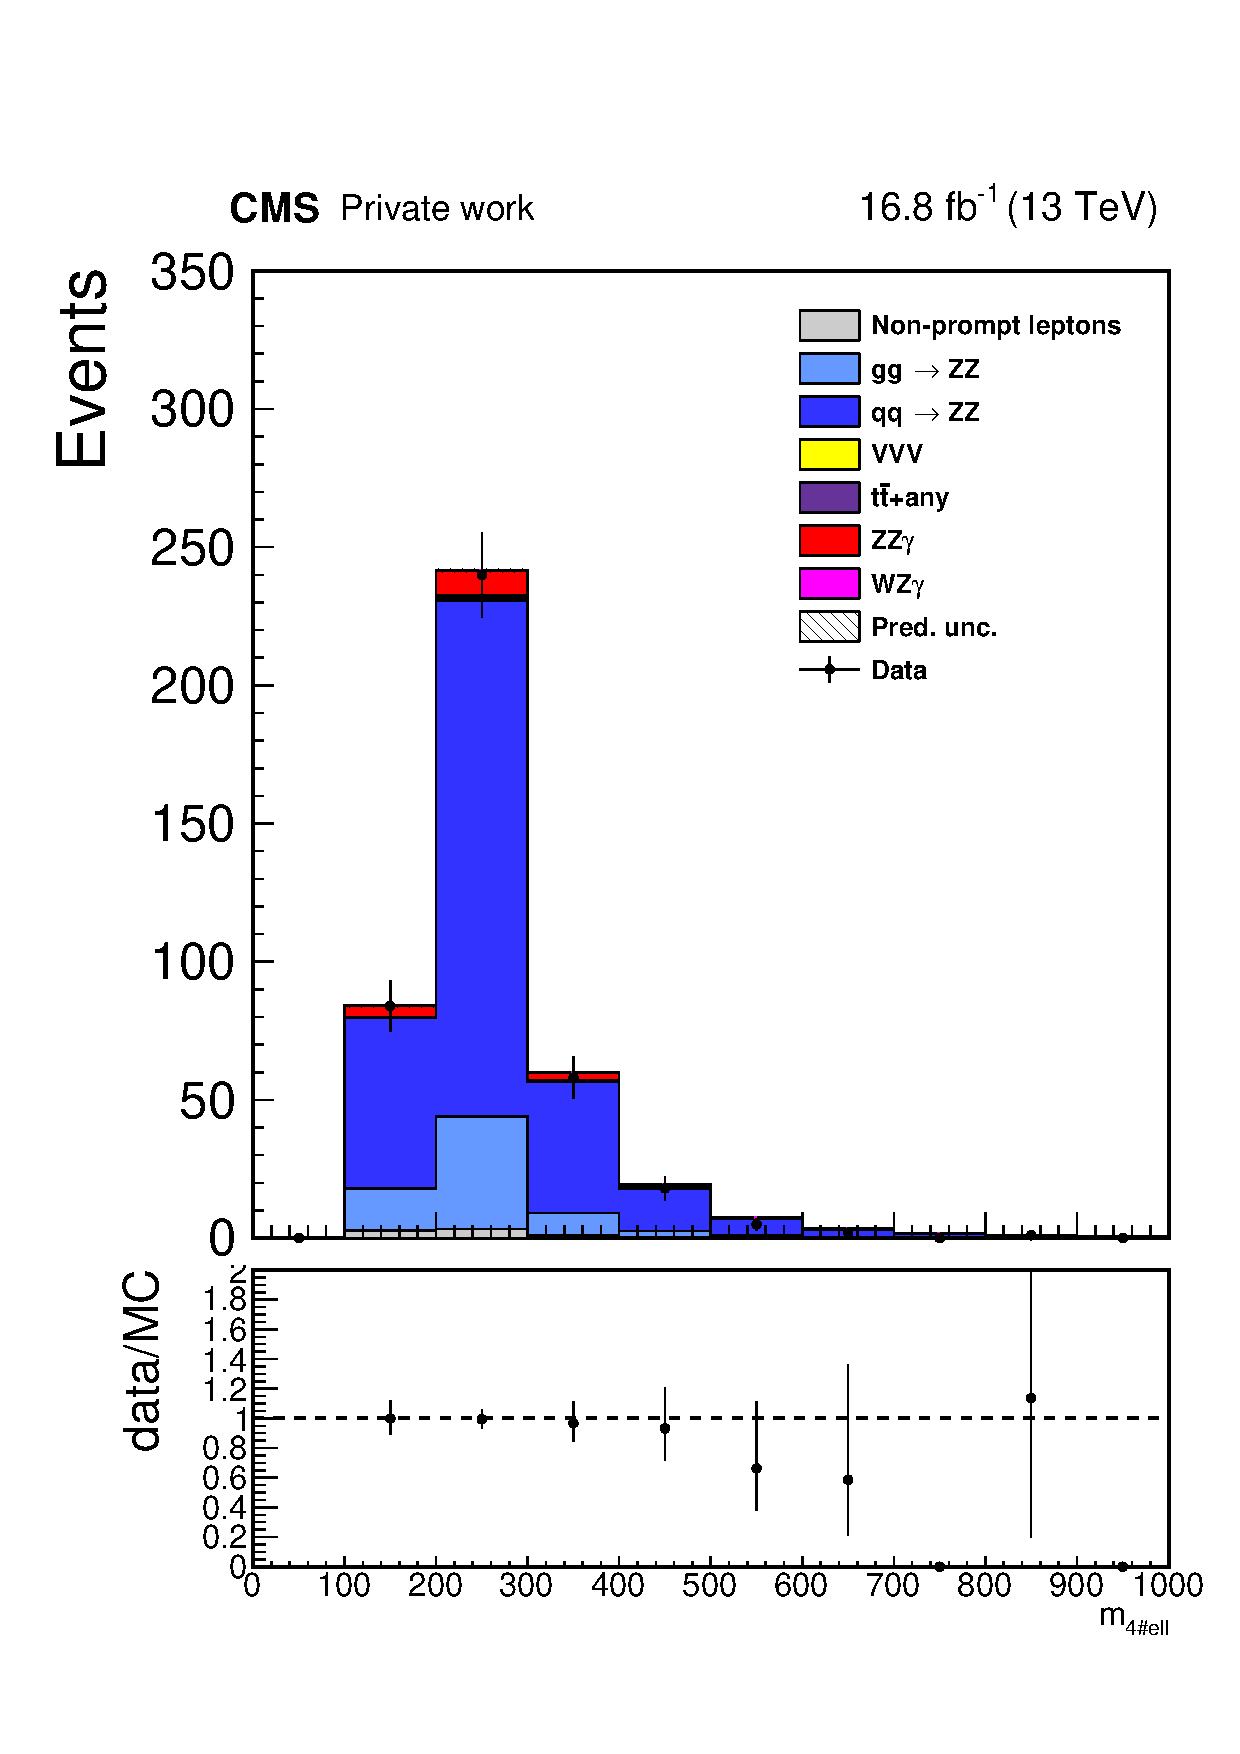
\includegraphics[width=.25\textwidth]{Figures/VVGammaAnalyzer/2016postVFP/lepCR/SR4P/ZZ_mass_pow.pdf}}%
\subfigure [2017       ] {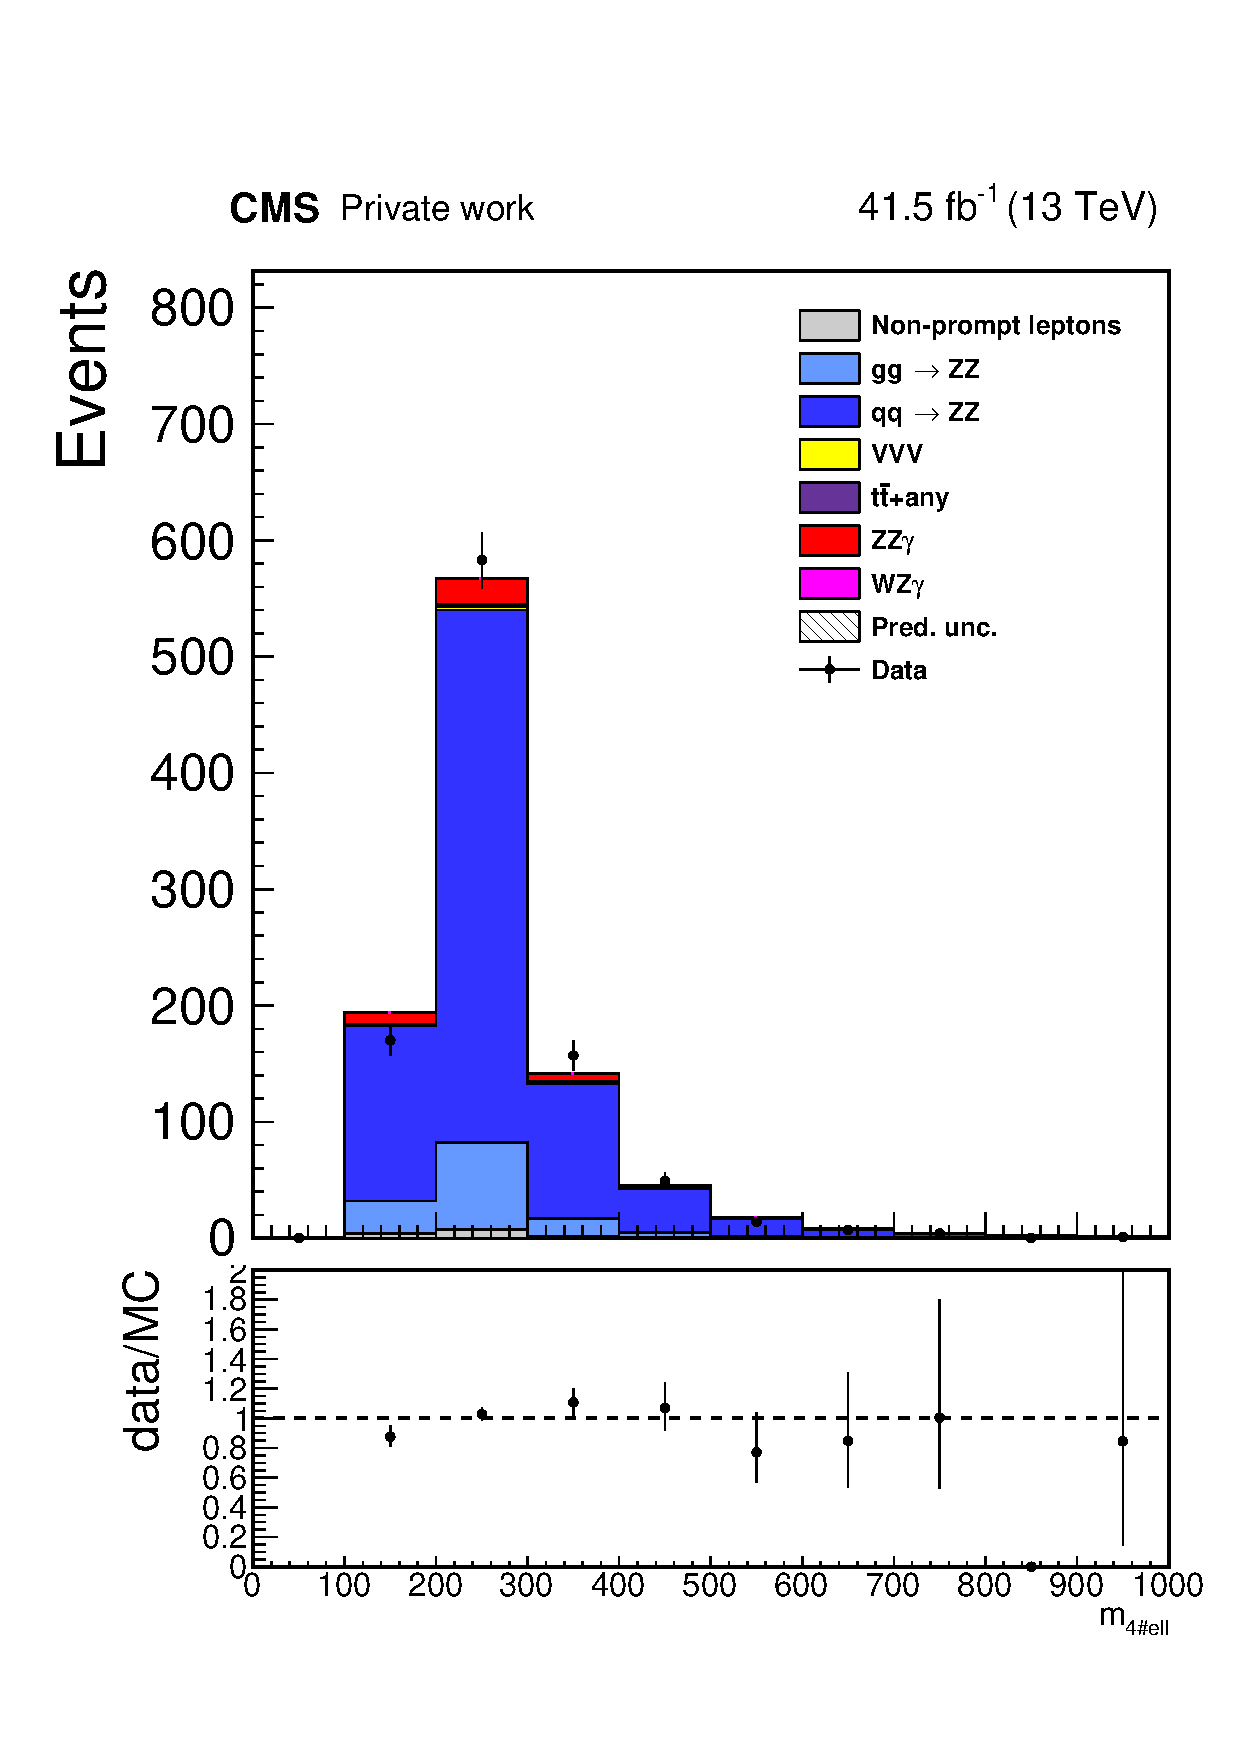
\includegraphics[width=.25\textwidth]{Figures/VVGammaAnalyzer/2017/lepCR/SR4P/ZZ_mass_pow.pdf}}%
\subfigure [2018       ] {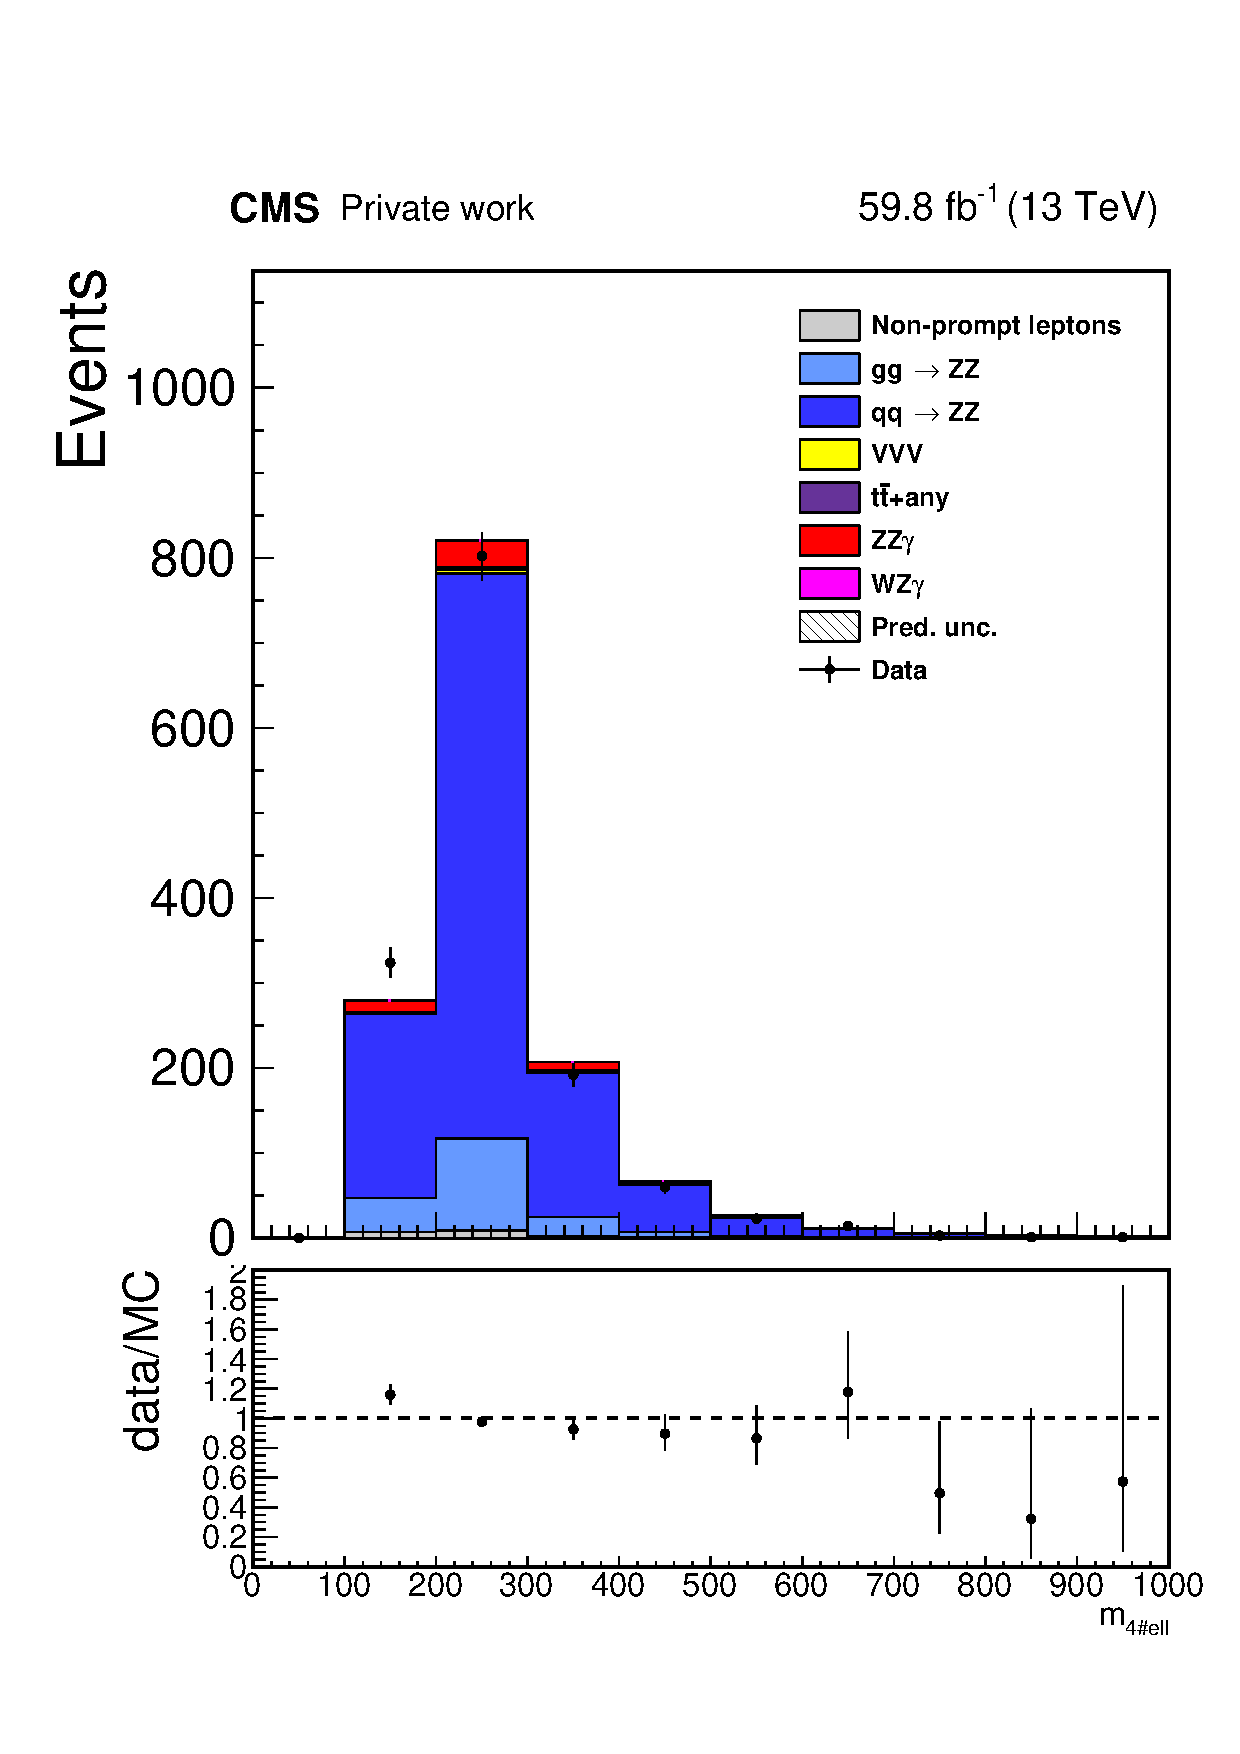
\includegraphics[width=.25\textwidth]{Figures/VVGammaAnalyzer/2018/lepCR/SR4P/ZZ_mass_pow.pdf}}
\caption{Invariant mass of the ZZ system, without any requirements on the presence of photons, for each of the data-taking periods of Run2.}
\label{fig:ZZmass_byyear}
\end{figure}

\section{Statistical analysis}
\label{sec:statistical_analysis}
The likelihood function is defined as the Probability Density Function for a set of parameters of a model, given a certain set of experimental observables (data).
The model adopted for this analysis defines a signal strength modifier $\mu$, that multiplies the cross section of the $ZZ\gamma$ signal and leaves all the other processes unchanged.
Each independent source of systematic uncertainty descrbed in \todo{ref{sec:systematics}} is assigned a nuisance parameter $\theta_i$, and the full set is denoted $\vec\theta$.
They are of no direct interest for this analysis, but must be considered in the fitting procedure to extract correct results.
They enter the model through their PDF $p_i(\tilde{\theta_i}|\theta_i)$, which is the probability of measuring a certain value of the parameter given that the true value is $\theta_i$.
Furthermore, the expected yields of background, $b$, and signal, $s$, depend on the value of the nusance parameters.

The global likelihood function is thus defined as:
\begin{equation}
  \label{eq:likelihood_full}
  \Likelihood(data\, |\, \mu, \vec\theta\,) = \prod_c \Likelihood_c(data\, |\, \mu \cdot s(\vec\theta\,) + b(\vec\theta\,)) \cdot \prod_i p_i(\tilde{\theta_i}\, |\, \theta_i)
\end{equation}
where c runs over all the channels, which are the four data-taking periods (2016preVFP, 2016postVFP, 2017, 2018).
The extraction of the signal strength proceeds through the maximization of the complete likelihood function by varying the parameter of interest $\mu$ and the nuisances.
The $\Likelihood_c$ functions are the PDF of the binned distributions in each channel, and are given by the product of Poisson probabilities for every bin $j$ to observe $n_j$ events:
\begin{equation}
  \label{eq:likelihood_bin}
  \Likelihood_c(data\, |\, \mu \cdot s(\vec\theta\,) + b(\vec\theta\,)) = \prod_j \frac{\mu \cdot s_j(\vec\theta\,) + b_j(\vec\theta\,)}{n_j!} e^{-(\mu \cdot s_j(\vec\theta\,) + b_j(\vec\theta\,))}
\end{equation}

\subsection{Treatment of nuisance parameters}
Systematics uncertainties can be categorized into two main classes: the ones that affect only the event yield, and those that have an impact also on the shape of the predicted distributions.
Most of the uncertainties of the first class are parametrised with a log-normal distribution:
\begin{equation}
  \label{eq:lnNdef}
  \Probability(\tilde{\theta}\,|\,\theta) = \frac{1}{\sqrt{2 \pi} \text{ln} k} \cdot \frac{1}{\tilde{\theta}} \cdot \text{exp} \left( -\frac{(\text{ln}(\tilde{\theta}/\theta_m))^2}{2 \text{ln}^2 k} \right)
\end{equation}
which is the distribution of a random variable whose logarithm is normally distributed, with mean $\mu$ = $\text{ln}(\theta_m)$ and standard deviation $\sigma$ = $\text{ln}(k)$.
%% where the parameters $theta_s$ and $k$ can be defined in terms of the mean and standard deviation of a normally distributed variable: $\theta_m = e^{\mu}$ and $k = e^{\sigma}$.
The log-normal is used instead of a gaussian because it enforces the positive-definite normalization for the nuisance modeled, which is usually multiplying an event yield and thus cannot be negative.

The remaining systematics in the first class are those that represent a background coming from a statistically limited control region, such as the fake leptons and photons.
These are dominated by the statistically uncertainty in the control region and are modelled with a Gamma distribution:
\begin{equation}
  \label{eq:gammadef}
  \Probability(\theta\,|\,N\alpha) = \frac{1}{\Gamma(N) \alpha^N} \theta^{N-1} e^{-\theta/\alpha}
\end{equation}
where $N$ is the number of events in the control region, $\theta$ is the average transfer factor and $\Gamma(x)$ is the Gamma function.

The shape uncertainties of the second class are accounted for by interpolating the event fraction for each bin of three histograms: the one obtained for the central value, and the two obtained by shifting the nuisance parameter up and down by one standard deviation.

\subsection{Quantifying an excess}
To quatify the statistical significance of an excess of events over the background-only hypotesis, the following test statistic is used:
\begin{equation}
  \label{eq:test_statistic}
  t_0 = -2\text{ln} \frac {\Likelihood(data\,|\,0,\widehat{\vec{\theta_0}}\,)} {\Likelihood(data\,|\,\hat\mu,\widehat{\vec\theta}\,)}\,,\quad \text{with}\, \hat\mu \ge 0
\end{equation}

The numerator is evaluated under the background-only hypothesis ($\mu$ = 0), and $\widehat{\vec{\theta_0}}$ is the set of values of nuisance parameters that maximises it under this null hypothesis.
The denominator is evaluated under the alternative signal + background hypothesis, and the values $\hat{\mu}$ and $\hat{\vec{\theta}}$ are those that maximise the likelihood in this hypotesis.
This quantity is positive for a signal-like excess ($\mu$ > 0) and becomes 0 in the absence of an excess ($\mu$ = 0).

The significativity of an excess is expressed in terms of the local \textit{p-value}, which is the probability to obtain a value of the test statistic $t_0$ greater than or equal to the one observed in experimental data, under the background-only hypothesis:
\begin{equation}
  \label{eq:pvalue}
  p_0 = \Probability(t_0 \ge t_0^{obs}\, |\, \mu = 0)
\end{equation}
That is, $p_0$ is the probability that a local statistical fluctuation of the background resembles the signal at least as much as the observed data do.

The p-value is usually expressed as a \textit{significance} $Z$ using the Gaussian one-sided integral:
\begin{equation}
  \label{eq:significance}
  p_0 = \int_Z^\infty \frac{1}{\sqrt{2\pi}}e^{-x^2/2}dx
\end{equation}

The conventional values of $Z$ = 3$\sigma$ and $Z$ = 5$\sigma$, corresponding to p-values of $1.3 \cdot 10^{-3}$ and $2.8 \cdot 10^{-7}$, are used to claim evidence for and the discovery of a new phenomenon respectively.
